\section{Progettazione concettuale}

\subsection{Descrizione entità e relazioni} 
\subsubsection[Entità ed attributi]{Entità ed attributi \protect\footnote{Gli identificatori delle entita' sono indicati dal simbolo $\blacklozenge$ mentre gli altri attributi sono indicati dal simbolo $\lozenge$}}

%\begin{multicols}{2} 
%\begin{flushleft}


\textbf{Negozio}: 
\setlist{nolistsep}
\begin{itemize}
\item [ $\blacklozenge$]ID : string
\item [$\lozenge$]Indirizzo : string 
\item[$\lozenge$]Citta : string
\end{itemize}

\textbf{Magazzino}:
\begin{itemize}[noitemsep]
\item [$\blacklozenge$] ID : string
\item [$\lozenge$] Indirizzo : string
\item [$\lozenge$] Citta : string
\item [$\lozenge$] Volume : int
\end{itemize}

\textbf{Componente}:
\begin{itemize}
\item [$\blacklozenge$] ID : string
\item [$\lozenge$] Nome : string
\item [$\lozenge$] Prezzo : float
\item [$\lozenge$] Tipo : enum\{SM,CPU,SV,Cooler,RAM,Mem,Case,Alim\}
\end{itemize}
Dove SM = scheda madre, SV = scheda video, Mem = memoria, Alim = alimentatore.\\

%\columnbreak
\textbf{Produttore}:
\begin{itemize}
\item [$\blacklozenge$] Nome : string
\item [$\lozenge$] Email : string
\item [$\lozenge$] Telefono : string
\end{itemize}

\textbf{PC}:
\begin{itemize}
\item [$\blacklozenge$] Nome : string
\item [$\lozenge$] Prezzo : float
\item [$\lozenge$] Funzione : enum\{Ufficio, Gaming, Grafica e design\}
\end{itemize}

\textbf{Dipendenti}:
\begin{itemize}
\item [$\blacklozenge$] CF : string
\item [$\lozenge$] Nome : string
\item [$\lozenge$] Cognome : string
\item [$\lozenge$] Data : date
\item [$\lozenge$] Stipendio : int 
\end{itemize}
I dipendenti si suddividono in Commessi, Manutentori e Consulenti, ognuno dei quali non ha bisogno di informazioni aggiuntive per essere rappresentato.

%\columnbreak
\textbf{Cliente}:
\begin{itemize}
\item [$\blacklozenge$] ID : string
\item [$\lozenge$] Nome : string 
\item [$\lozenge$] Cognome : string
\item [$\lozenge$] Email : string
\end{itemize}

\textbf{Acquisto}:
\begin{itemize}
\item [$\blacklozenge$] ID : string
\item [$\lozenge$] Totale : float
\item [$\lozenge$] Data : date
\end{itemize}
Gli acquisti a loro volta si suddividono in acquisti che riguardano componenti o che riguardano pc gia' assemblati. Gli acquisti di componenti poi si suddividono in acquisti conclusi e non conclusi. Cio' per rappresentare il fatto che se alcuni componenti dovessero mancare in magazzino, il cliente puo' procedere con l'ordinazione di quest'ultimi.


\textbf{Ordine}:
\begin{itemize}
\item [$\blacklozenge$] ID : int
\item [$\lozenge$] Date\_ordine : date
\item [$\lozenge$] Data\_arrivo : date
\end{itemize}

\textbf{Manutenzione}:\footnote{L'entità ha un identificatore esterno con l'entità manutentore}
\begin{itemize}
\item [$\blacklozenge$] ID\_manutentore : string
\item [$\blacklozenge$] Data : timestamp
\item [$\lozenge$] Tipo : enum\{Riparazione, Assemblaggio\}
\item[$\lozenge$] Durata : time
\end{itemize}

%\end{flushleft}
%\end{multicols}

\subsubsection{Relazioni}
\begin{itemize}

\item[$\blacksquare$] \underline{Negozio - Magazzino} : \textbf{disponibilità}
\begin{itemize}
\item[$\square$] Ogni negozio dispone di un singolo magazzino
\item[$\square$]Un magazzino rifornisce un singolo negozio
\end{itemize}

\item[$\blacksquare$]\underline{Negozio - Dipendente} : \textbf{impiego}
\begin{itemize}
\item[$\square$]Ciascun negozio ha almeno un dipendente
\item[$\square$]Un dipendente lavora in un singolo negozio
\item[$\square$]Il negozio può avere più di un dipendente
\end{itemize}

\item[$\blacksquare$]\underline{Negozio - Acquisto} : \textbf{registro}
\begin{itemize}
\item[$\square$]Il negozio può non aver registrato alcun acquisto o averne registrati molteplici
\item[$\square$]Ogni acquisto viene identificato da un id univoco tra i negozi, percui può essere fatto da un negozio solo
\end{itemize}

\item[$\blacksquare$]\underline{Magazzino - Componente} : \textbf{contenuto}
\begin{itemize}
\item[$\square$]Un magazzino contiene da 0 a molti componenti
\item[$\square$]Un componente può essere contenuto in più magazzini
\end{itemize}

\item[$\blacksquare$]\underline{Componente - Produttore} : \textbf{fornitura}
\begin{itemize}
\item[$\square$]Ciascun componente è prodotto e fornito da un produttore
\item[$\square$]Un produttore produce e fornisce almeno un componente
\end{itemize}

\item[$\blacksquare$]\underline{Componente - PC} : \textbf{configurazione}
\begin{itemize}
\item[$\square$]Piu' componenti formano la configurazione di un pc 
\item[$\square$]Un componente puo' essere inserito in piu' di un pc
\end{itemize}

\item[$\blacksquare$]\underline{Consulente - Cliente} : \textbf{consulenza}
\begin{itemize}
\item[$\square$]Un consulente puo' non aver effettuato consulenze o averne effettuate molte
\item[$\square$]Un cliente puo' aver ricevuto nessuna consulenza oppure diverse
\end{itemize}

\item[$\blacksquare$]\underline{Manutentore - Manutenzione} : \textbf{esecuzione}
\begin{itemize}
\item[$\square$]Un manutentore ha la possibilita' di eseguire piu' manutenzioni o anche nessuna
\item[$\square$]Una manutenzione deve essere eseguita da un manutentore
\end{itemize}

\item[$\blacksquare$]\underline{Manutenzione - Cliente} : \textbf{richiesta}
\begin{itemize}
\item[$\square$]Una manutenzione e' richiesta da un cliente
\item[$\square$]Un cliente puo' richiedere da 0 a molte manutenzioni
\end{itemize}

\item[$\blacksquare$]\underline{Acquisto - Cliente} : \textbf{effettua}
\begin{itemize}
\item[$\square$]Ciascun acquisto e' realizzato da un cliente
\item[$\square$]Un cliente effettua almeno un acquisto e puo' farne anche molteplici
\end{itemize}

\item[$\blacksquare$]\underline{Acquisto - Commesso} : \textbf{registrazione}
\begin{itemize}
\item[$\square$]Un commesso registra da 0 a molti acquisti
\item[$\square$]Un acquisto e' registrato da un cliente
\end{itemize}

\item[$\blacksquare$]\underline{Acquisto(Componente) - Componente} : \textbf{composizione}
\begin{itemize}
\item[$\square$]Un acquisto di componenti e' composto da almeno un componente
\item[$\square$]Un componente puo' essere compreso in piu' di un acquisto o in nessuno
\end{itemize} 

\item[$\blacksquare$]\underline{Acquisto(Componente) Non concluso - Ordine} : \textbf{realizzazione}
\begin{itemize}
\item[$\square$]Un acquisto non concluso di un componente implica la realizzazione di un ordine
\item[$\square$]Un ordine e' realizzato a fronte di un singolo acquisto non concluso
\end{itemize}

\item[$\blacksquare$]\underline{Acquisto(Pre-assemblato) - PC} : \textbf{composizione}
\begin{itemize}
\item[$\square$]Un acquisto di un pc pre-assemblato e' composto da un singolo PC
\item[$\square$]Un PC puo' essere registrato o meno in un acquisto(pre-assemblato)
\end{itemize}

\item[$\blacksquare$]\underline{Ordine - Componente} : \textbf{riferimento}
\begin{itemize}
\item[$\square$]Un ordine riferisce a uno o piu' componenti
\item[$\square$]Un componente puo' essere riferito in piu' di un ordine o da nessuno
\end{itemize}


\end{itemize}

\subsection{Schema concettuale (E-R)}

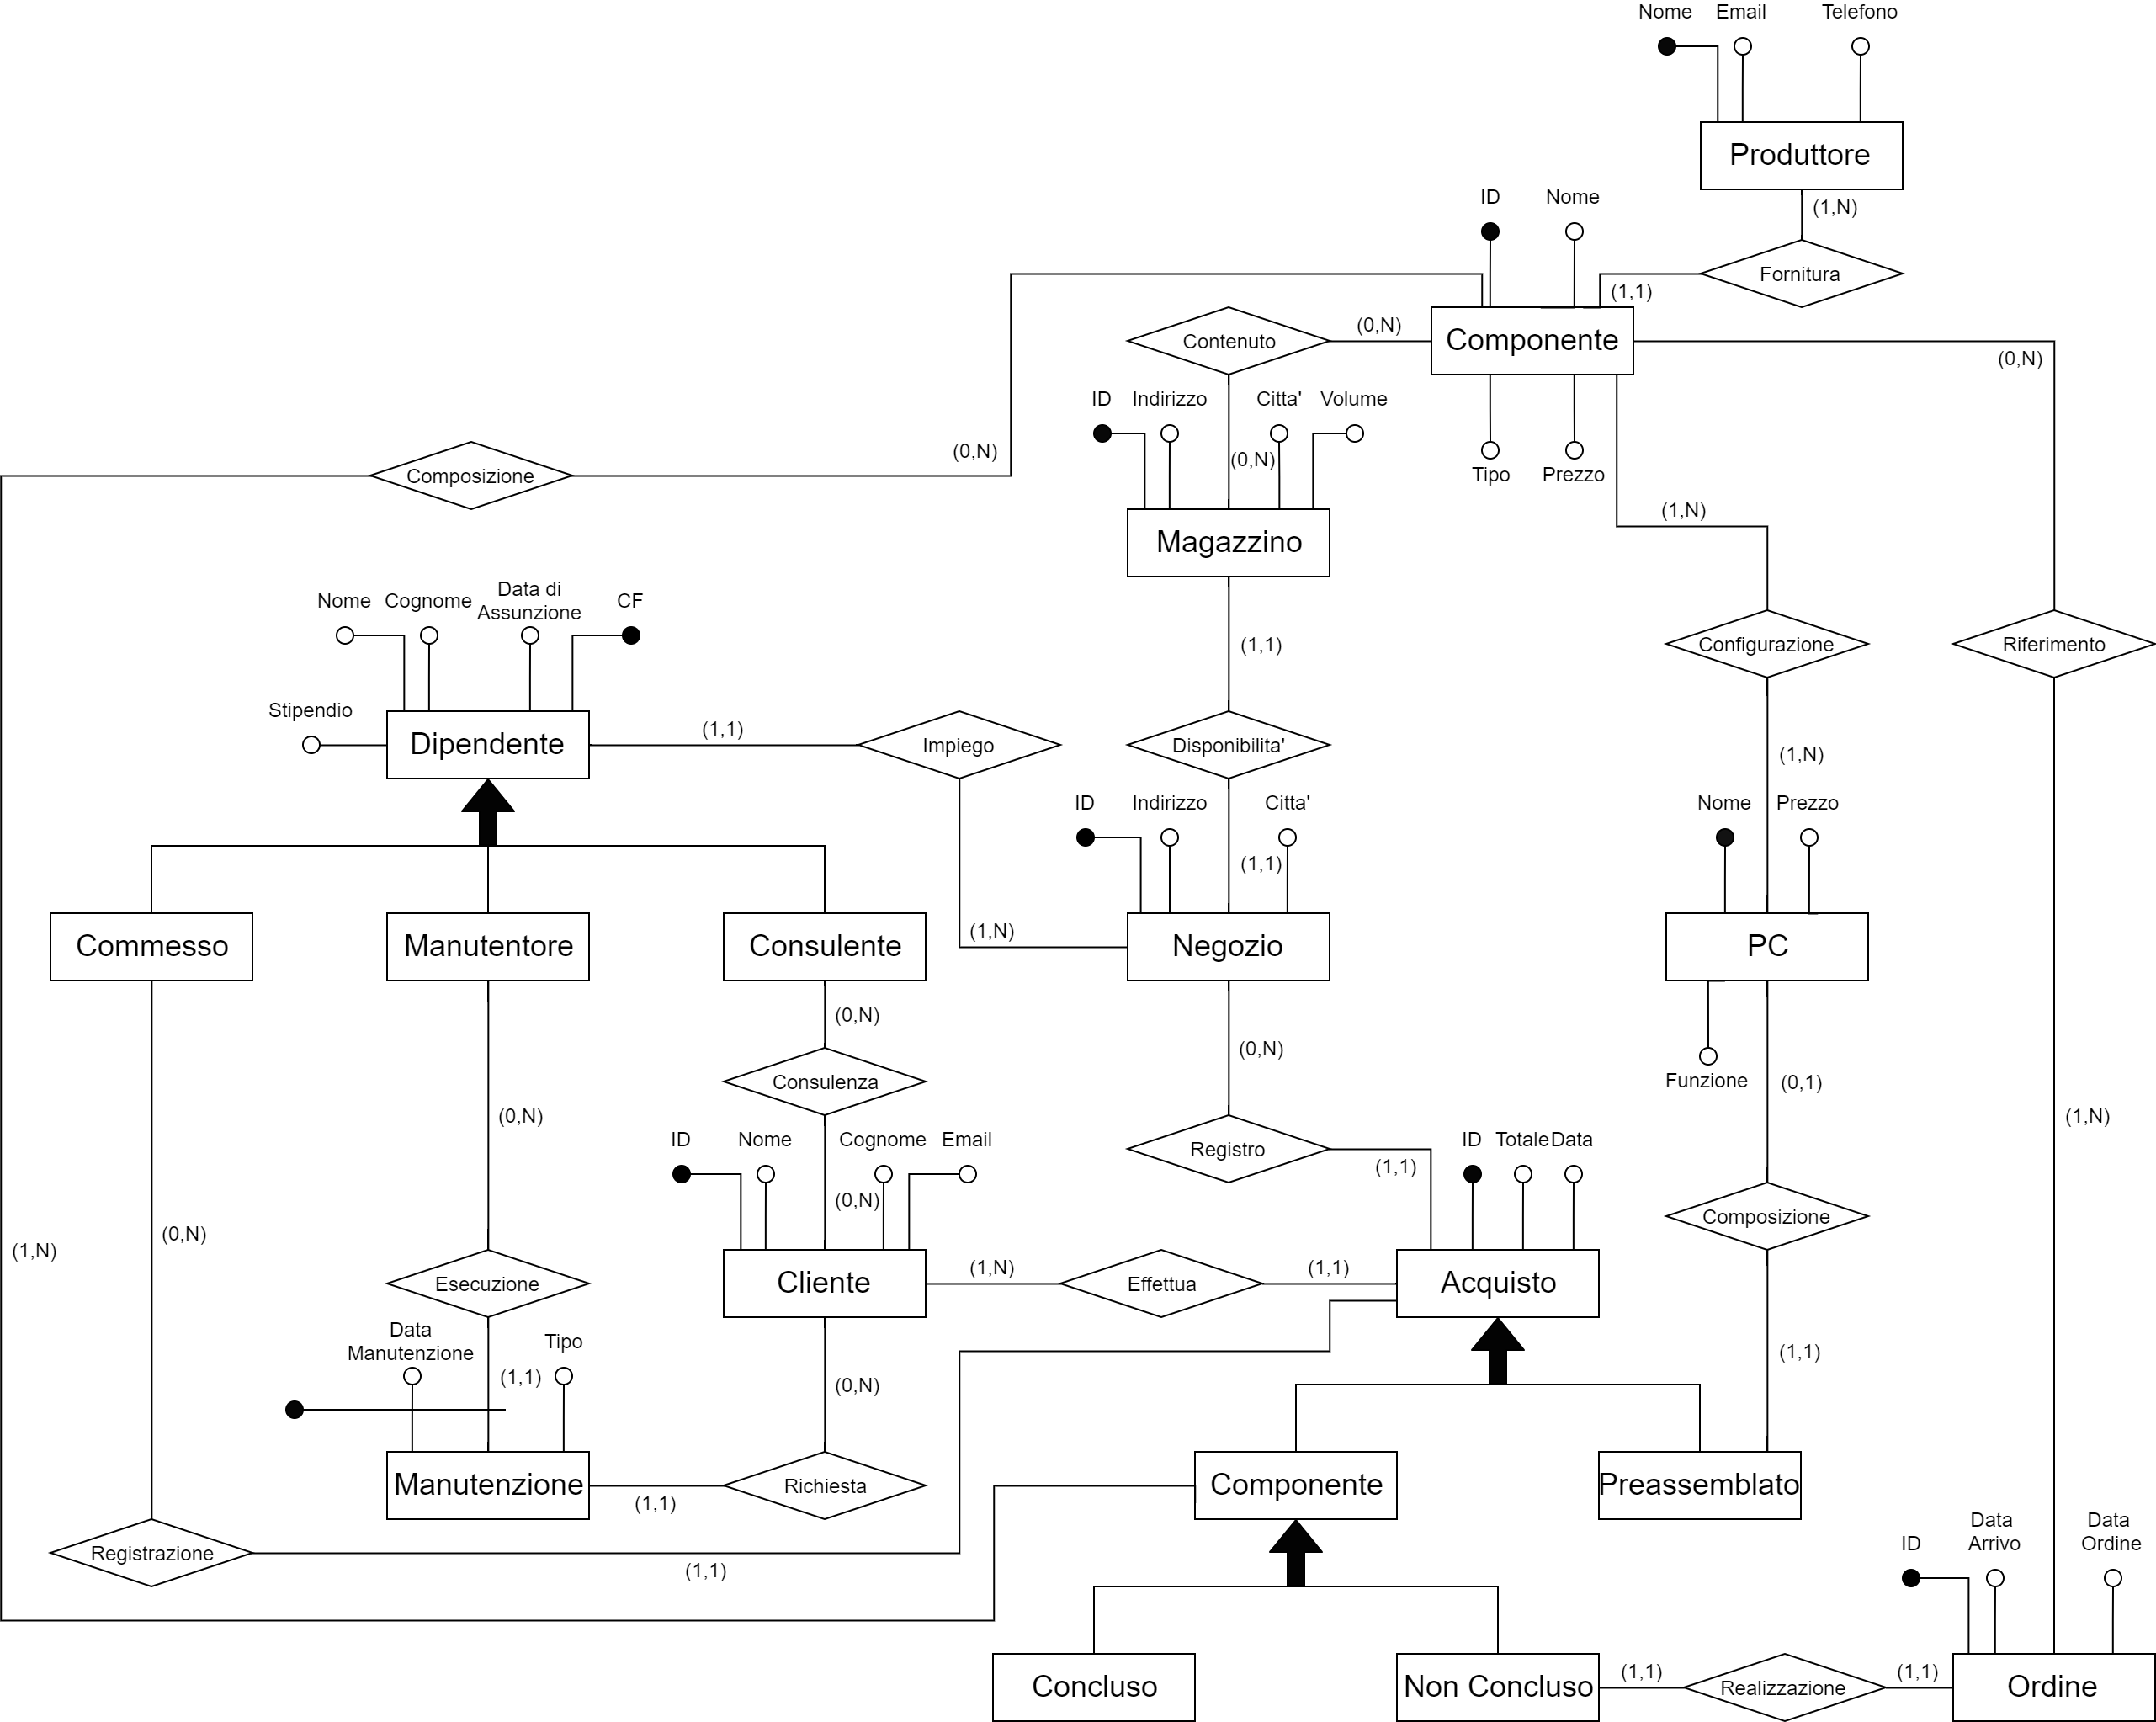
\includegraphics[width=\textwidth]{ER}
